\begin{figure}
	\centering
	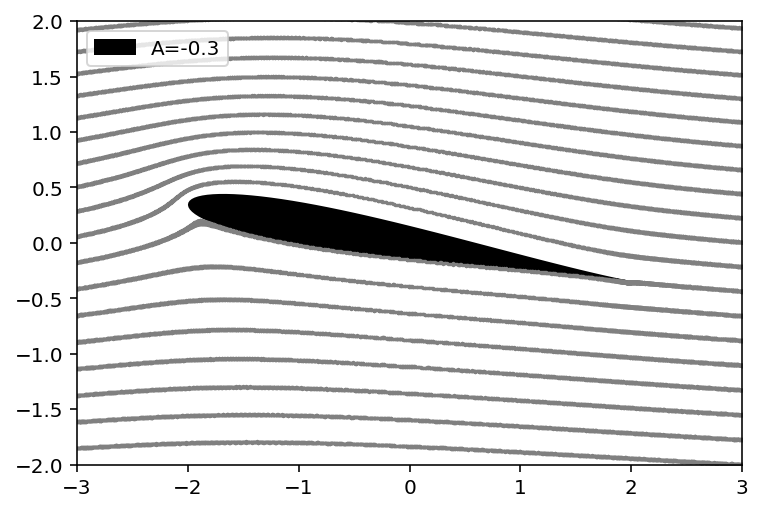
\includegraphics[width=0.6\textwidth]{papers/joukowski/images/05_stroemungslinien/fluegel_strom_A030_Rot_V02_g.png}
	\caption{
		Das Flügelprofil weist einen Anstellwinkel auf. Somit
		verschwindet die Symmetrie in den Strömungslinien und es entsteht eine Auftriebskraft,
		obwohl das Flügelprofil symmetrisch ist.
		\label{joukowski:Stroemungslinien:fig_fluegel2}
	}
\end{figure}
